%!TEX root = ../thesis.tex

\section{学習フェーズ}

  学習フェーズの概要を\figref{Fig:RobotGuidance_learning_system}に示す.学習フェーズでは,2DLiDARの反射強度を利用したルールベース制御器を用いて,\figref{Fig:RobotGuidance_learning_phase_leg}に示す追従対象者の足に装着した再帰反射テープに向かって,ロボットを制御する.ルールベース制御器の出力は,ロボットのヨ―方向の角速度$\omega$の1つとし,角速度$\omega$が0 \,[rad/s]となるようにロボットを制御することで人追従することが可能と考えられる.並行して,この行動とカメラの画像データを深層学習器に入力して,オンラインで学習させる.なお,並進速度は0.2 \,[m/s]で一定にしているため,深層学習器に入力しない.

  \begin{figure}[h]
    \centering
    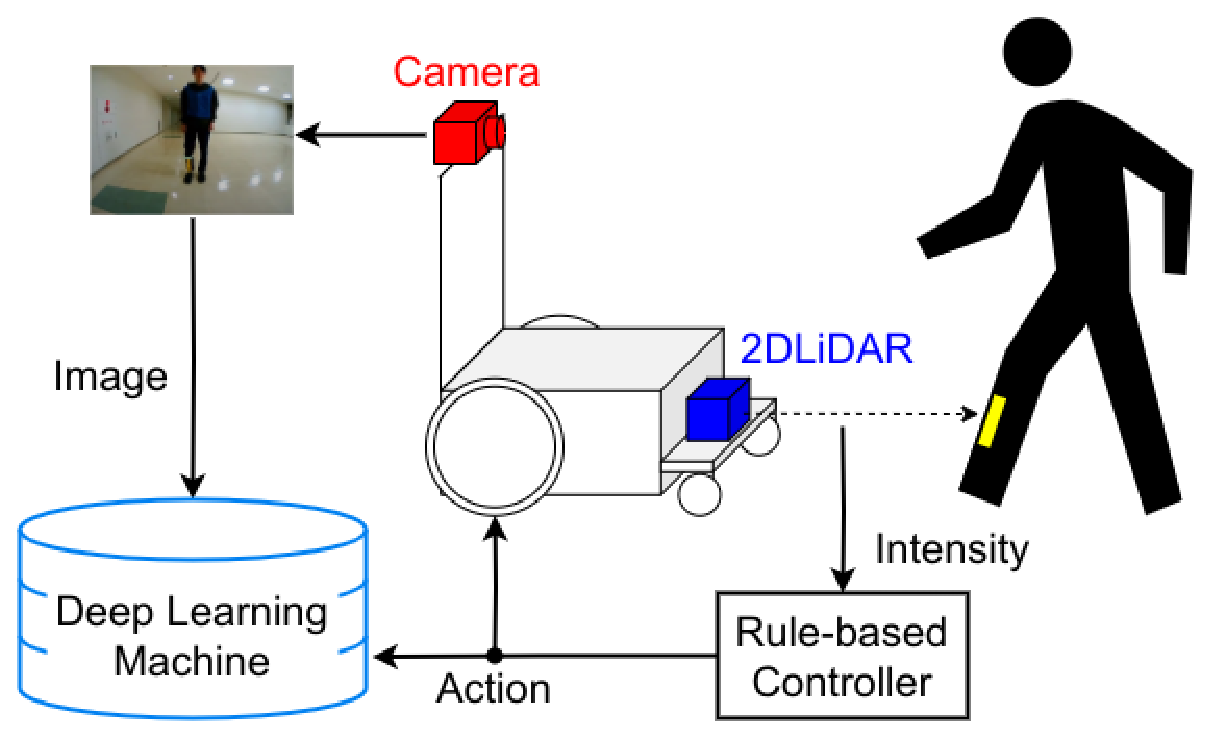
\includegraphics[keepaspectratio, scale=0.45] {images/eps/RobotGuidance_learning_system}
    \captionsetup{justification=raggedright} % キャプションを左寄せに
    \caption{Proposed method in the learning phase}
    \label{Fig:RobotGuidance_learning_system}
  \end{figure}

  \begin{figure}[h]
    \centering
    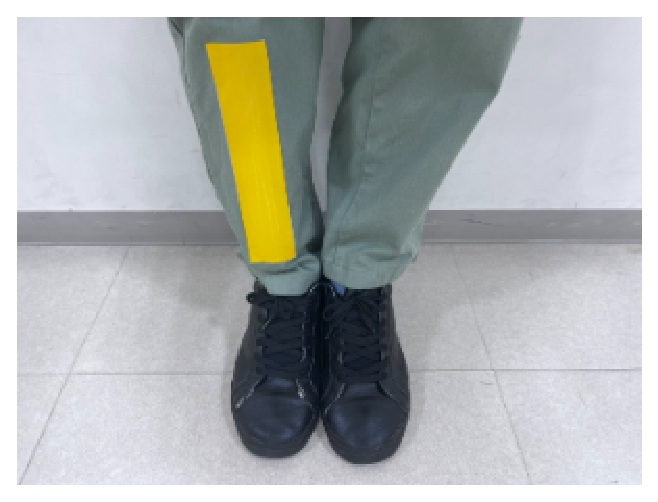
\includegraphics[keepaspectratio, scale=0.55] {images/eps/RobotGuidance_learning_phase_leg}
    \captionsetup{justification=raggedright} % キャプションを左寄せに
    \caption{Wearing retroreflective tape}
    \label{Fig:RobotGuidance_learning_phase_leg}
  \end{figure}

\newpage
